% SC2005 Ch02 — Processes and Threads (no \documentclass)
\chapter{Processes and Threads}
\label{ch:processes}

\begin{quote}
\emph{A process is a program in execution.} Understanding how the OS creates,
schedules, and isolates processes --- and how threads share within a process ---
is the foundation for concurrency.
\end{quote}

\noindent\textbf{Learning Outcomes.} After this chapter you will be able to:
\begin{enumerate}[label=(L\arabic*)]
  \item define process, PCB, and process states; explain context switching;
  \item use \texttt{fork}, \texttt{exec}, \texttt{wait}, and \texttt{exit};
  \item distinguish threads vs.\ processes and user vs.\ kernel threads;
  \item reason about multithreading models and pthreads programming;
  \item describe IPC mechanisms (pipes, shared memory, message passing).
\end{enumerate}

% ============================================================
\section{The Process Abstraction}
\label{sec:process-def}

A \emph{program} is passive (code on disk); a \emph{process} is active, with a
program counter, registers, address space (text/data/heap/stack), and OS
resources (open files, signals). Each process has a \emph{Process Control Block}
(PCB) storing PID, state, PC, registers, scheduling info, memory limits, open
files, and accounting.

\subsection{Process States}
\begin{center}
\textit{New} $\to$ \textit{Ready} $\to$ \textit{Running} $\leftrightarrow$
\textit{Waiting/Blocked} $\to$ \textit{Terminated}. The scheduler moves Ready
$\to$ Running (dispatch); I/O or \texttt{wait} moves Running $\to$ Waiting;
interrupt/completion moves Waiting $\to$ Ready.
\end{center}

\begin{figure}[h!]
\centering
\begin{tikzpicture}[scale=0.78, every node/.style={font=\small},
  st/.style={draw, rounded corners, align=center, minimum width=2.1cm, minimum height=0.85cm}]
  \node[st, fill=blue!12] (new) at (0,2.0) {New};
  \node[st, fill=green!14] (ready) at (3.6,2.0) {Ready};
  \node[st, fill=orange!18] (run) at (7.0,2.0) {Running};
  \node[st, fill=violet!12] (wait) at (7.0,0.1) {Waiting};
  \node[st, fill=gray!18] (term) at (3.6,0.1) {Terminated};
  \draw[-{Stealth}, thick, blue!60!black] (new) -- (ready) node[midway,above,font=\tiny]{admitted};
  \draw[-{Stealth}, thick, blue!60!black] (ready) -- (run) node[midway,above,font=\tiny]{dispatch};
  \draw[-{Stealth}, thick, red!60!black] (run) -- (wait) node[midway,right,font=\tiny]{I/O / wait};
  \draw[-{Stealth}, thick, green!50!black] (wait) -- (ready) node[midway,below,font=\tiny]{I/O done} ;
  \draw[-{Stealth}, thick] (run) -- ++(0,-0.55) -| (ready) node[pos=0.25,below,font=\tiny]{interrupt / yield};
  \draw[-{Stealth}, thick] (run) -- (term) node[midway,right,font=\tiny]{exit};
  \draw[-{Stealth}, thick, dashed] (new) -- (term);
\end{tikzpicture}
\caption{Five-state process model and transitions.}
\label{fig:proc-states}
\end{figure}

\subsection{Context Switch}
On a timer interrupt or blocking call, the kernel saves the running process's
registers/PC into its PCB, selects the next Ready process, restores its context,
and resumes. This is pure overhead --- no user work is done --- so fast
switching matters.

% ============================================================
\section{Process Creation: \texttt{fork} and \texttt{exec}}
\label{sec:fork-exec}

In UNIX, \texttt{fork()} creates a child that is a near-clone of the parent
(copy of address space with copy-on-write, duplicated file descriptors). It
returns $0$ in the child and the child's PID ($>0$) in the parent (or $-1$ on
failure). \texttt{exec*()} replaces the current image with a new program.

\begin{lstlisting}[language=C,caption={fork--exec--wait pattern (POSIX)}]
#include <unistd.h>
#include <sys/wait.h>
#include <stdio.h>
int main() {
    pid_t pid = fork();
    if (pid == 0) {
        // child
        execlp("ls", "ls", "-l", NULL); // replaces child image
        perror("exec"); _exit(1);
    } else if (pid > 0) {
        int status; waitpid(pid, &status, 0); // parent waits
        printf("child exited: %d\n", WEXITSTATUS(status));
    } else { perror("fork"); }
    return 0;
}
\end{lstlisting}

\texttt{wait}/\texttt{waitpid} lets a parent collect a child's exit status;
\texttt{exit(status)} terminates a process. An orphan is reaped by \texttt{init};
a zombie retains its PCB until the parent waits.

\begin{figure}[h!]
\centering
\begin{tikzpicture}[scale=0.74, every node/.style={font=\footnotesize},
  p/.style={draw, rounded corners, align=center, minimum width=2.4cm, minimum height=0.8cm}]
  \node[p, fill=blue!13] (par) at (0,2.0) {Parent\\ \texttt{PID=100}};
  \node[p, fill=green!14] (c1) at (-2.2,0.4) {Child\\ \texttt{PID=101}};
  \node[p, fill=orange!14] (c2) at (2.2,0.4) {Child\\ \texttt{PID=102}};
  \node[p, fill=violet!12] (g1) at (-2.2,-1.1) {Grandchild\\ \texttt{PID=103}};
  \draw[-{Stealth}, thick, blue!60!black] (par) -- (c1) node[midway,left,font=\tiny]{fork};
  \draw[-{Stealth}, thick, blue!60!black] (par) -- (c2) node[midway,right,font=\tiny]{fork};
  \draw[-{Stealth}, thick, green!50!black] (c1) -- (g1) node[midway,left,font=\tiny]{fork};
  \node[font=\tiny, align=left] at (3.8,-1.1) {Copy-on-write\\address space};
\end{tikzpicture}
\caption{Process tree formed by successive \texttt{fork} calls.}
\label{fig:fork-tree}
\end{figure}

% ============================================================
\section{Threads}
\label{sec:threads}

A \emph{thread} is a schedulable unit within a process: it has its own PC,
registers, and stack, but shares text, data, heap, and open files with peer
threads. Benefits: responsiveness, resource sharing, economy (cheaper to create
than a process), and parallelism on multicore.

\subsection{User vs.\ Kernel Threads}
\textit{User threads} are managed by a library (fast switch, but a blocking
syscall blocks the whole process). \textit{Kernel threads} are OS-managed
(heavier, but independently schedulable). Hybrid \textit{many-to-many} maps
$m$ user threads onto $n$ kernel threads.

\subsection{Pthreads Example}
\begin{lstlisting}[language=C,caption={POSIX threads: parallel sum}]
#include <pthread.h>
#include <stdio.h>
#define N 1000000
long sum = 0; pthread_mutex_t lk = PTHREAD_MUTEX_INITIALIZER;
void *worker(void *arg) {
    long lo = ((long*)arg)[0], hi = ((long*)arg)[1];
    long local = 0;
    for (long i = lo; i < hi; i++) local += i;
    pthread_mutex_lock(&lk); sum += local; pthread_mutex_unlock(&lk);
    return NULL;
}
int main() {
    pthread_t t1, t2; long r1[]={0,N/2}, r2[]={N/2,N};
    pthread_create(&t1,NULL,worker,r1);
    pthread_create(&t2,NULL,worker,r2);
    pthread_join(t1,NULL); pthread_join(t2,NULL);
    printf("sum=%ld\n", sum);
    return 0;
}
\end{lstlisting}

\begin{figure}[h!]
\centering
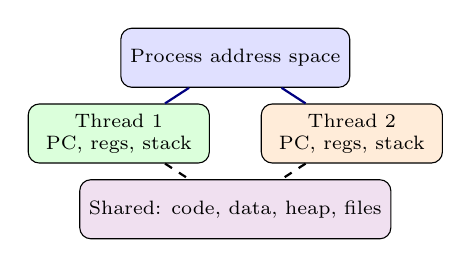
\begin{tikzpicture}[scale=0.74, every node/.style={font=\scriptsize},
  b/.style={draw, rounded corners, align=center, minimum width=2.3cm, minimum height=0.75cm}]
  \node[b, fill=blue!12] (proc) at (0,2.0) {Process address space};
  \node[b, fill=green!14] (t1) at (-2.0,0.7) {Thread 1\\PC, regs, stack};
  \node[b, fill=orange!15] (t2) at (2.0,0.7) {Thread 2\\PC, regs, stack};
  \node[b, fill=violet!12] (shared) at (0,-0.6) {Shared: code, data, heap, files};
  \draw[thick, blue!50!black] (proc) -- (t1); \draw[thick, blue!50!black] (proc) -- (t2);
  \draw[thick, dashed] (t1) -- (shared); \draw[thick, dashed] (t2) -- (shared);
\end{tikzpicture}
\caption{Single process, two threads sharing address space.}
\label{fig:threads}
\end{figure}

\subsection{IPC}
Cooperating processes need IPC: \textbf{pipes} (\texttt{pipe}), \textbf{shared
memory} (\texttt{shmget}/\texttt{mmap} + synchronization), and
\textbf{message passing} (\texttt{msgsnd}/\texttt{msgrcv}, sockets).

% ============================================================
\begin{remark}[Copy-on-write]
After \texttt{fork}, parent and child share physical pages read-only. Only on
a write does the kernel copy the page, making \texttt{fork} cheap even for
large address spaces. \texttt{exec} then discards the copied mapping entirely.
\end{remark}

\section{Exercises}
\label{sec:ch02-ex}
\begin{exercise}
Draw the PCB contents. Which fields must be saved on a context switch and why?
\end{exercise}
\begin{exercise}
What does the following print? Explain copy-on-write.
\begin{lstlisting}[language=C]
int x=10; if (fork()==0) { x++; printf("child %d\n",x); }
else { wait(NULL); printf("parent %d\n",x); }
\end{lstlisting}
\end{exercise}
\begin{exercise}
Compare processes vs.\ threads on isolation, creation cost, and communication.
When would you choose each?
\end{exercise}
\begin{exercise}
Explain many-to-one, one-to-one, and many-to-many thread models and their
trade-offs for blocking I/O and parallelism.
\end{exercise}
\begin{exercise}
Write a program where parent and child communicate via a pipe: child sends a
message, parent prints it.
\end{exercise}
